\begin{post}
	\postdata{You know you are in Tokyo when...}{2011}{11}{01}{00}{05}{23}
	\begin{content}	
\subsection{...the banner at the airport says "Welcome to Japan"}
(well, technically, this only means that you came to Japan, but whatever)	

\subsection{...a panda in a cape tells you not to put your hands into the doors}
\begin{figure}[!h]
\centering
{\fbox{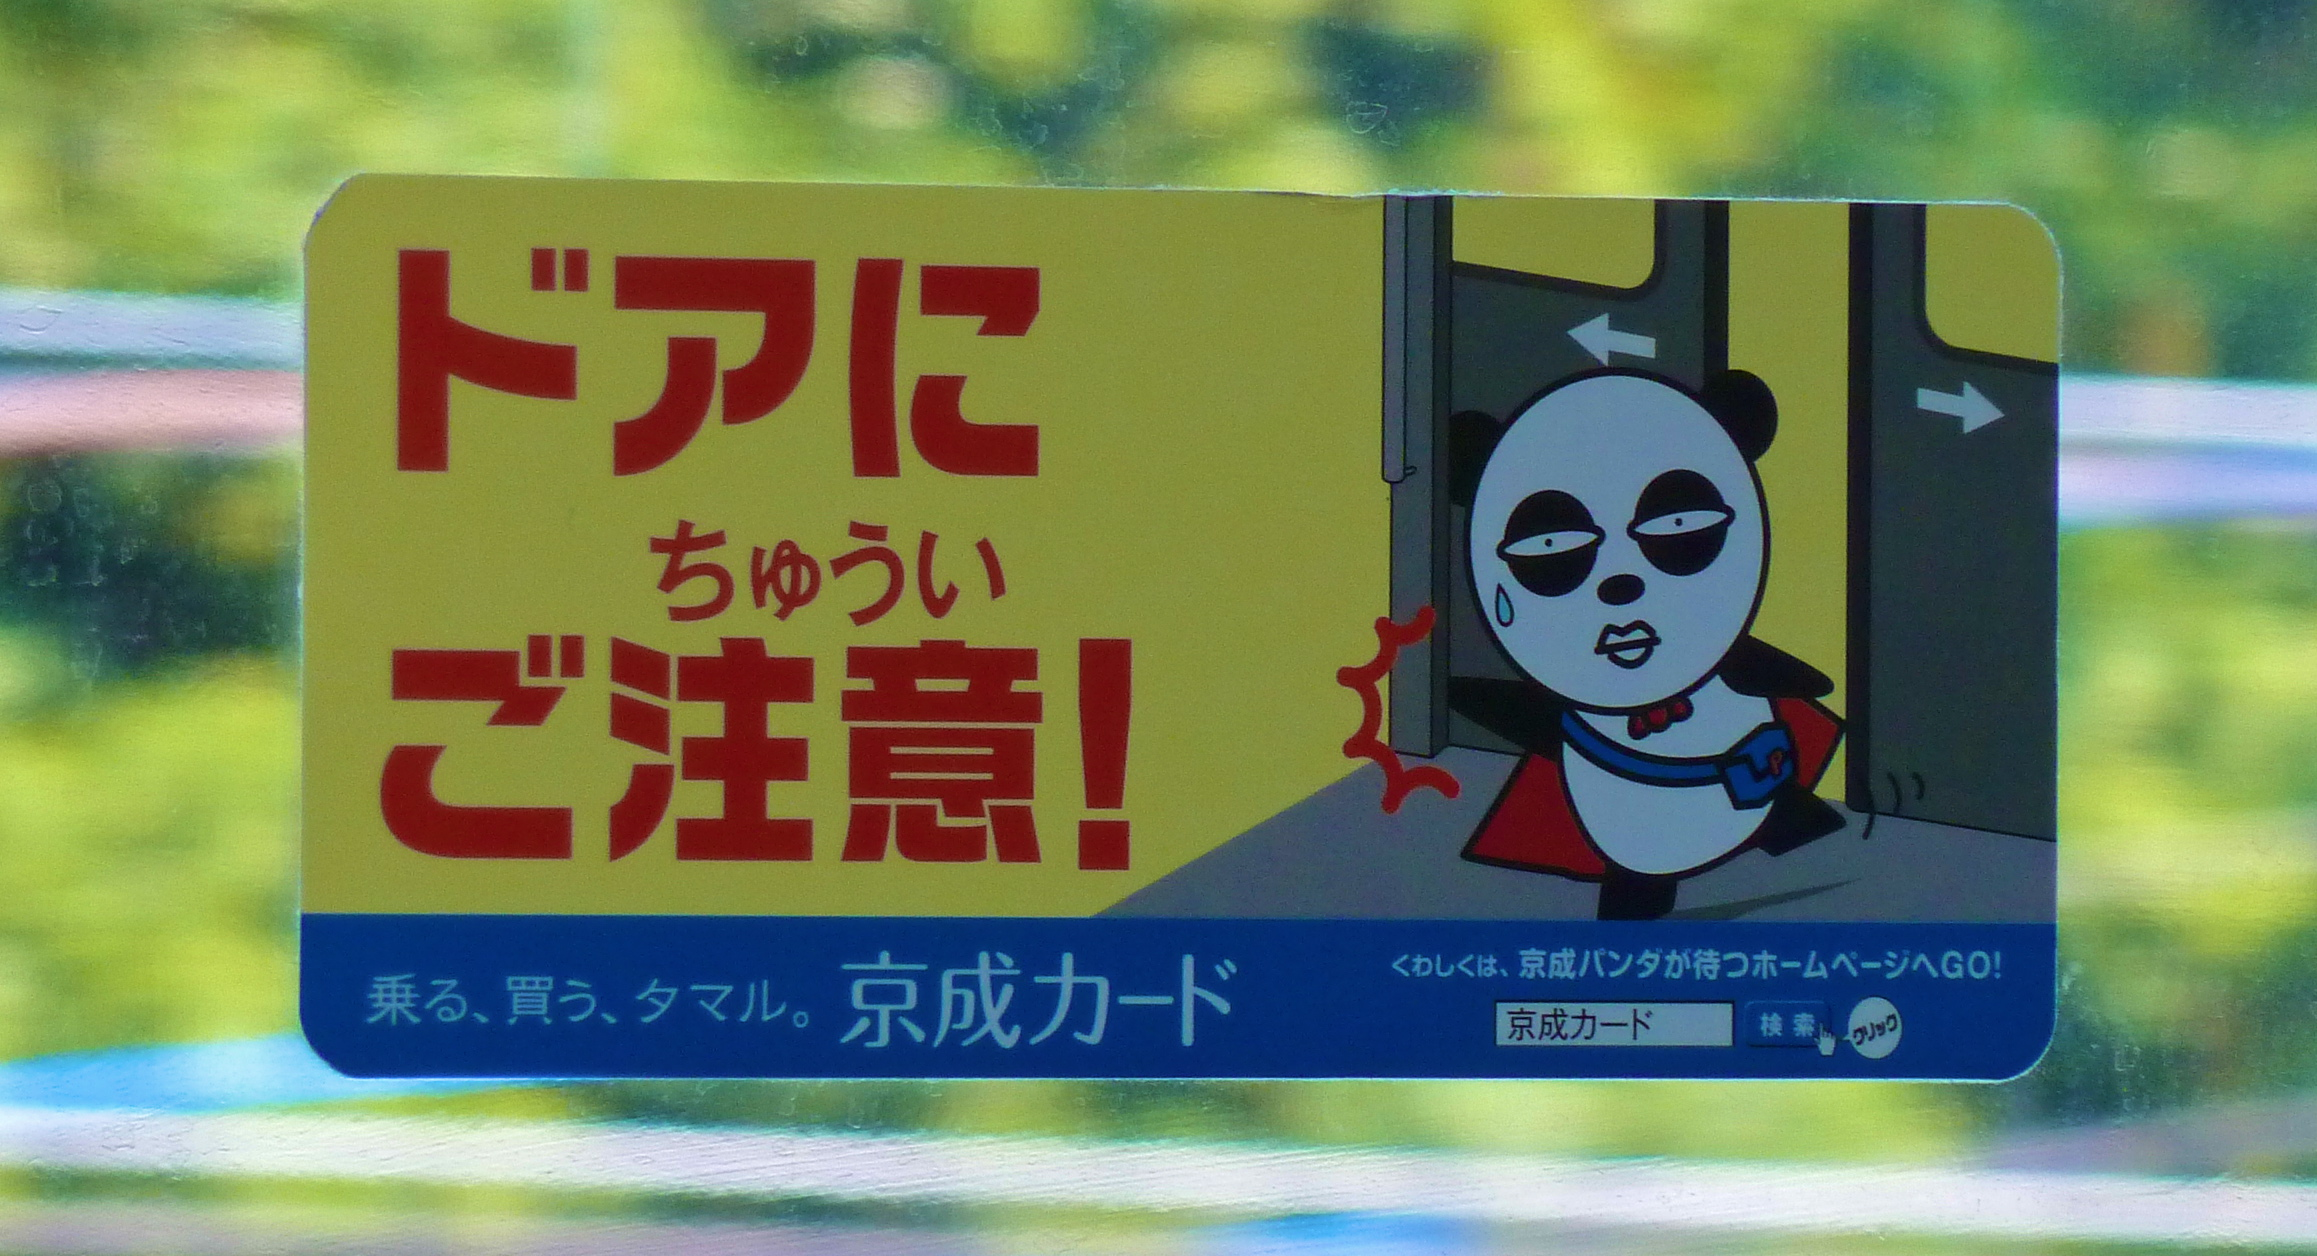
\includegraphics[width=0.6\textwidth]{photos/11/01/p10009941.jpg}}}
\end{figure}

\subsection{...talking on the phone in the subway is highly discouraged.}
It is not prohibited, but they politely ask you to <em>"refrain from talking on your mobile phone"</em>. I would not risk a ninja cutting my ear...

\subsection{...the subway system map is one big clusterfuck.}
\begin{wrapfigure}{r}{0.6\textwidth}
\vspace{-12pt}
\centering\fbox{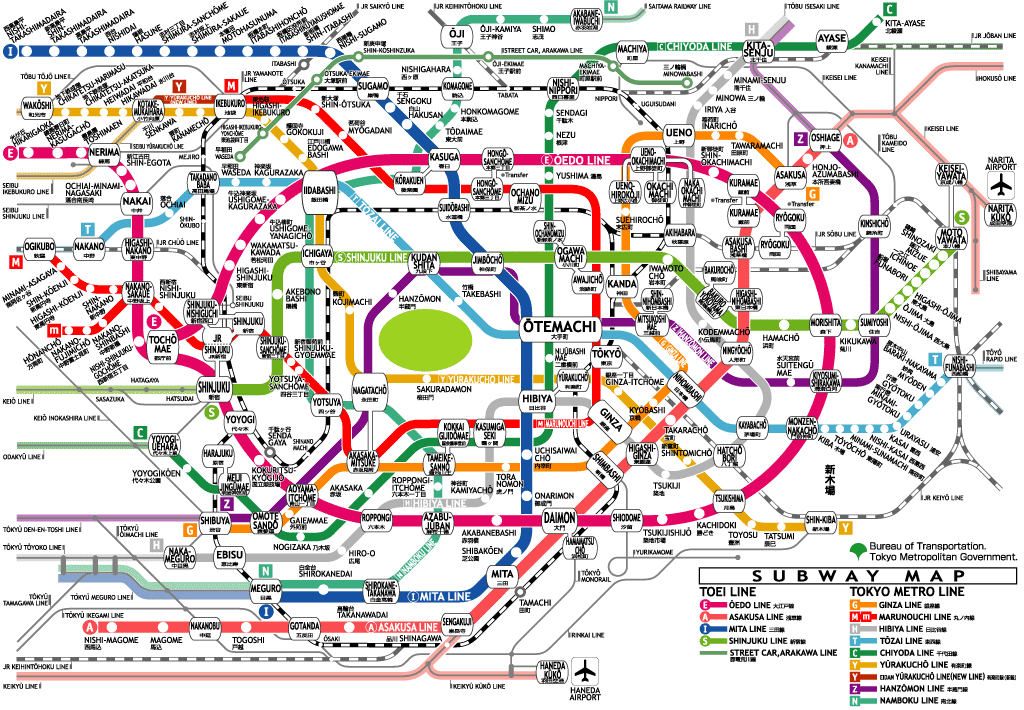
\includegraphics[width=0.6\textwidth]{photos/11/01/TokyoSubwayMap.png}}
\vspace{-24pt}
\end{wrapfigure}Seriously, that shit does not make sense! While normal subway maps try to at least partially display the real layout, in Tokyo, it is neatly arranged without much connection to reality (OK, not entirely, but it is just laid out in a weird manner). The problem is also the duality of the transport system there. Firstly, there are the \sout{Subway} Tokyo Metro and Toei, which represent the (mostly) underground parts. Secondly, there is the JR East part, which is a combination of regular trains (even Shinkansen) and commuter trains. These two parts can be used for transport in Tokyo, and in many cases you can transfer between subway and JR, but the maps quite often show either the JR or the subway system. At least they announce the other lines in the train's PA as well.

\subsection{...everything is more expensive than in Seoul. }
I knew that it is going to be expensive, but still, you are unpleasantly surprised when you find out that is really is. Take transportation as example. Upon arrival, we bought a Suica card, which is an alternative to the T-Money card used in Korea. It was pre-charged with ¥1500 of credit, which is approx. €15. We thought that it would be enough for the whole trip, because in Seoul charging 10,000KRW (= €6.60) is usually enough for up to two weeks. We were wrong — we had to recharge already the second day, and we haven't even used the card for the trip from the airport (¥1400, in Seoul approx. 3500-4000KRW). In total, I spent around €50 only for transport that weekend.

\subsection{...taxis are extremely expensive}
\begin{wrapfigure}{l}{0.5\textwidth}
\vspace{-12pt}
\centering{\fbox{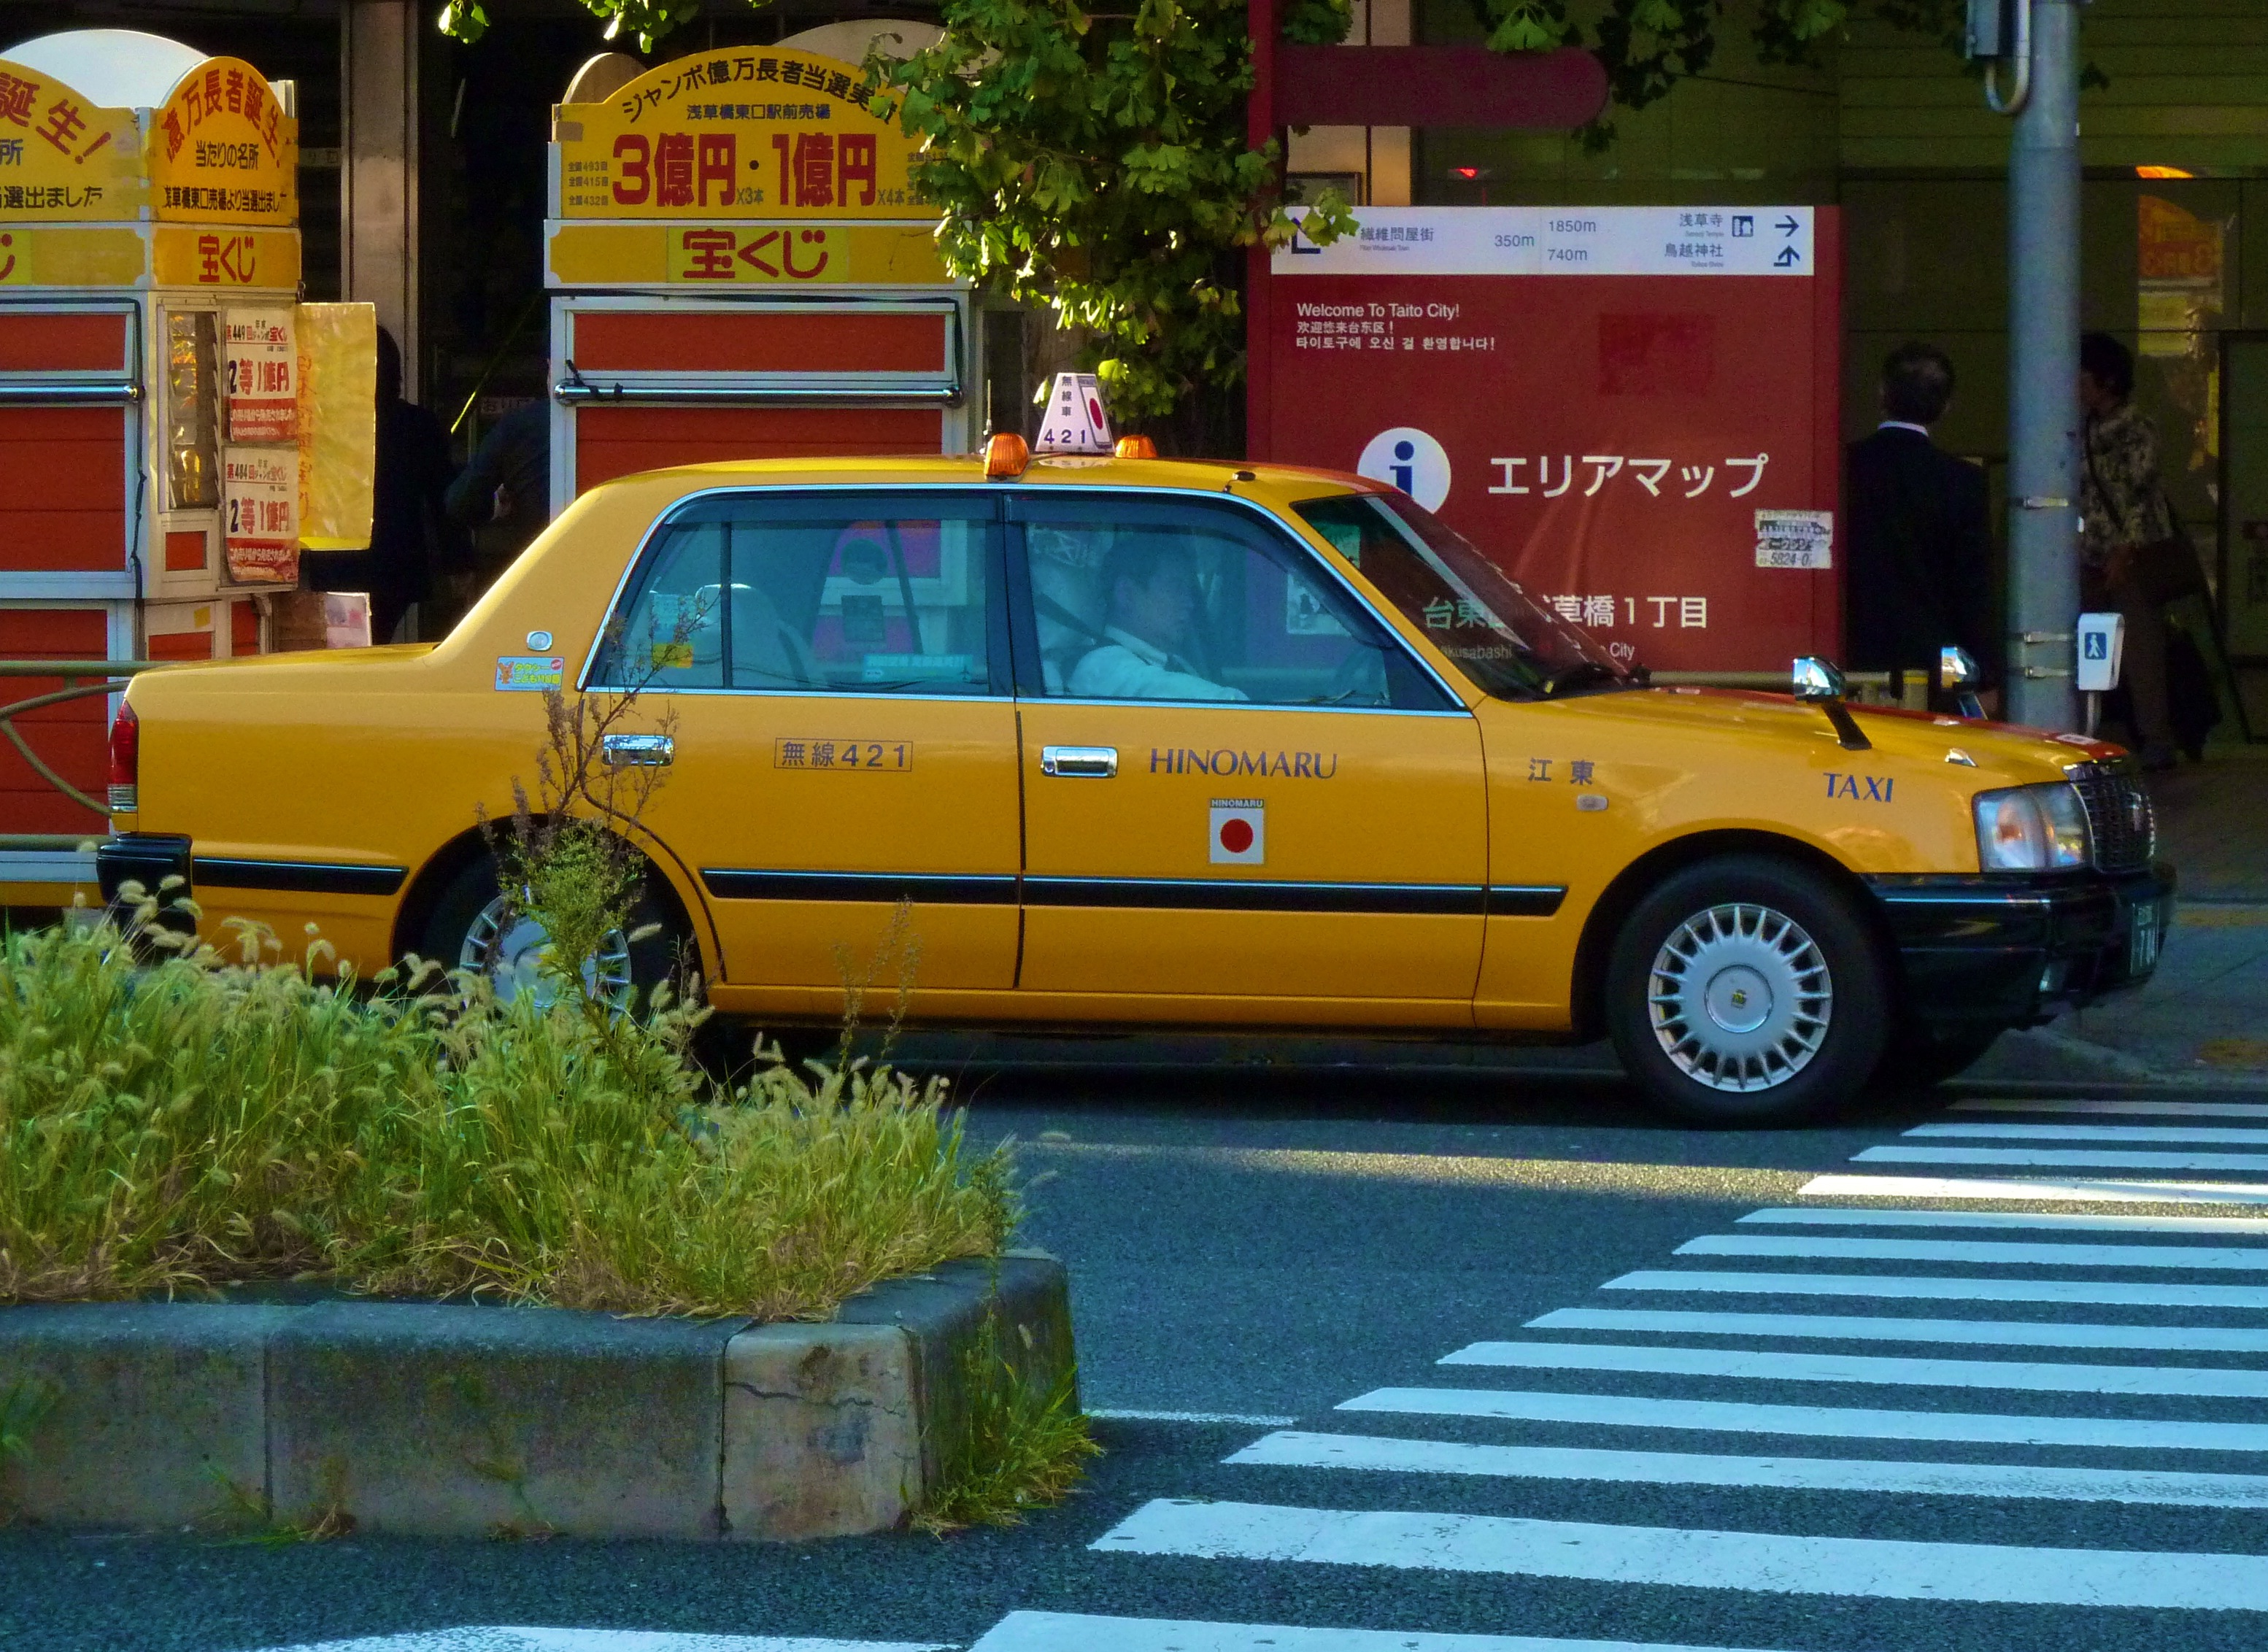
\includegraphics[width=0.5\textwidth]{photos/11/01/p10100171.jpg}}}
\vspace{-24pt}
\end{wrapfigure}Talking about money, due unforeseen events (mixing up the trains and taking the last train in the opposite direction) we had to take a taxi from Kamata to Shibuya. This approx. 30 minute ride set us back with staggering €60 bill, which meant €20 per person. The most I have paid for a taxi in Seoul so far was €5 for a 40 minute ride at 5am from Hongdae. The funny thing is that in Tokyo, the increment per unit is 100, which is the same as in Seoul. Won is, however, worth 10 times less than Yen. Sad story...

The (only) funny part is that the taxis are ooooooooold. They really stand out between all the modern cars, and maybe their age is the reason for the price. Repairing a 20yr old Nissan must be quite financially demanding.

\subsection{...girls are not wearing skirts.}
Technically, they are. But it does not seem so, since their skirts are merely belts. Well, I think I have even seen a wider belt. We were surprised despite being used to Korean girls, that dress up in heels and miniskirts even for taking out the trash. These nanoskirts, combined with knee-high socks and a lot of makeup makes Japanese girls look like dolls. Or <del>sluts </del> prostitutes, you choose. I guess it's just the culture, but it is quite funny when you see such girl walk with her mother (even young girls dress like that) and no one seems to care. No judging looks or remarks, slutty girls are simply part of the society. Not that we would complain about that, but it just feels weird.

\subsection{...you go to a Maid Café.}
This is one of the things that you somehow expect to see in Japan. It is weird, it is crazy, it is to some extent perverted and regular Japanese would never go there. Maid Café is a café, where you are waited by girls dressed as French maids, with short skirts and in many cases with little tails and ears. Seriously. Even though it sounds like something I just made up, Akihabara is full of such café, which are targeted at Otaku, Japanese nerds (often grown man) that like anime and manga, and a French maid is one of their biggest fantasies. Don't ask me why. These guys go to these café, drink, eat, talk to their waitress, that really treat them like their master.

%[caption id="" align="aligncenter" width="495" caption="Maids from a Maid Café (source: http://cryosites.com)"]<img title="Maid Café" src="http://www.cryosites.com/shared/img/m/maid_fnddh.jpeg" alt="Maid Café" width="495" height="329" />[/caption]

We got caught by a maid directly on the street, and since we wanted to go to a café anyway, we went with her. She was German, but assured us that she is the only non-Asian there, which made us feel even creepier than before. In the café, we got seated, received water and waited. Since this particular café did not have any cover charge (they normally do), the prices were higher than one would expect (coffee €6, beer €15). Their specialty was an omelette, on which they drew a picture with ketchup.

\begin{wrapfigure}{l}{0.32\textwidth}
\centering{\fbox{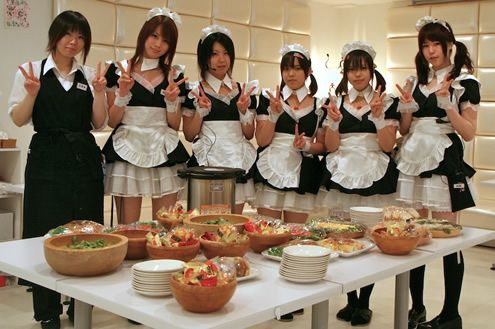
\includegraphics[height=103pt]{photos/11/01/maid.jpg}}}
\vspace{-24pt}
\end{wrapfigure}

I have to admit that the whole experience was quite uncomfortable. Even though at first we thought that it is hilarious, over the time we begun to feel creepy and perverted, watching these young-ish girls in their short dresses, talking to older Japanese guys. Btw. before leaving we found out that during their tour, even Backstreet Boys came to this café to see maids and have a cup of coffee and an omelette. Well, I don't want it that way.

\subsection{...people use three alphabets and you can't understand either of them.}
Kenji, Hiragana, Katakana. Each one has different purpose and looks different. In real world, they are, however mixed up together, so one word or phrase can contain all three of them. Thanks God for Hangul!

\subsection{...everything is überclean.}
The Japanese pursuit for perfection is materialized in the cleanness of streets, cars, buildings and the environment in general. Since almost everybody has a job in Japan (unemployment rate < 5\%), some people simply clean the streets and everything. I don't know if it's simply because there are more cleaners than in other countries, people do not litter that much or the cleaners are perfectionists, but the streets in particular look like they have been cleaned with a vacuum cleaner. Even the traffic signs on the road look fresh and new. I really admire that, because what you can sometimes see here in Seoul is quite gross. Well, cultural difference is cultural difference:)

\subsection{...you sometimes feel like you are a part of a big freak show.}
Even though we did not see the masses of cosplay people at Harajuku, the above pictures speak for themselves.\begin{figure}[!h]
\centering
\subfigure{\fbox{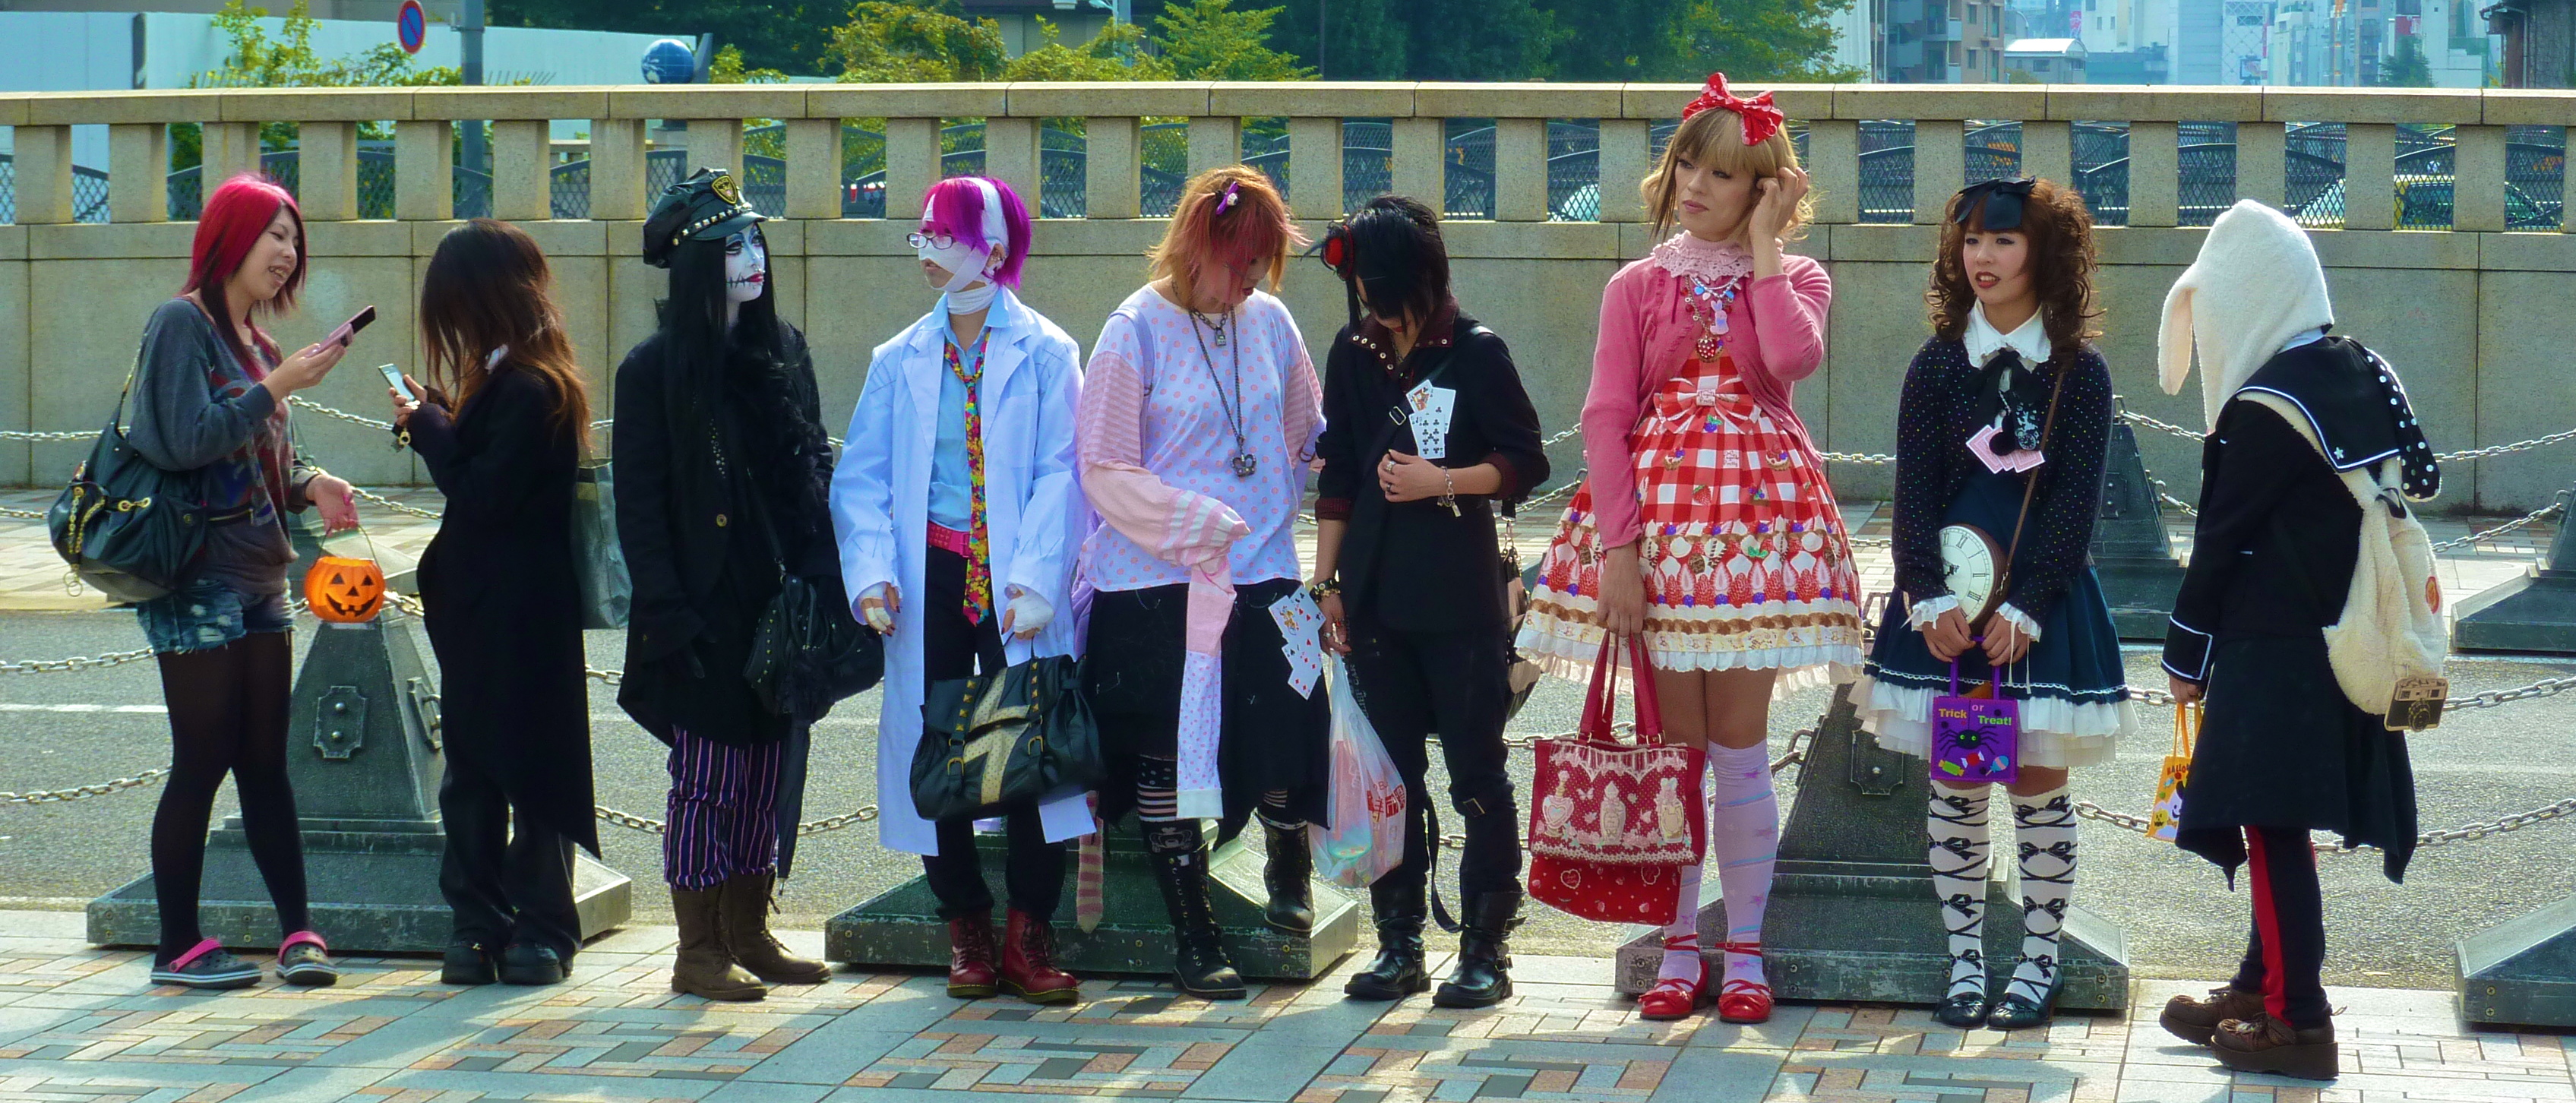
\includegraphics[height=0.25\textwidth]{photos/11/01/p10101751.jpg}}}
\subfigure{\fbox{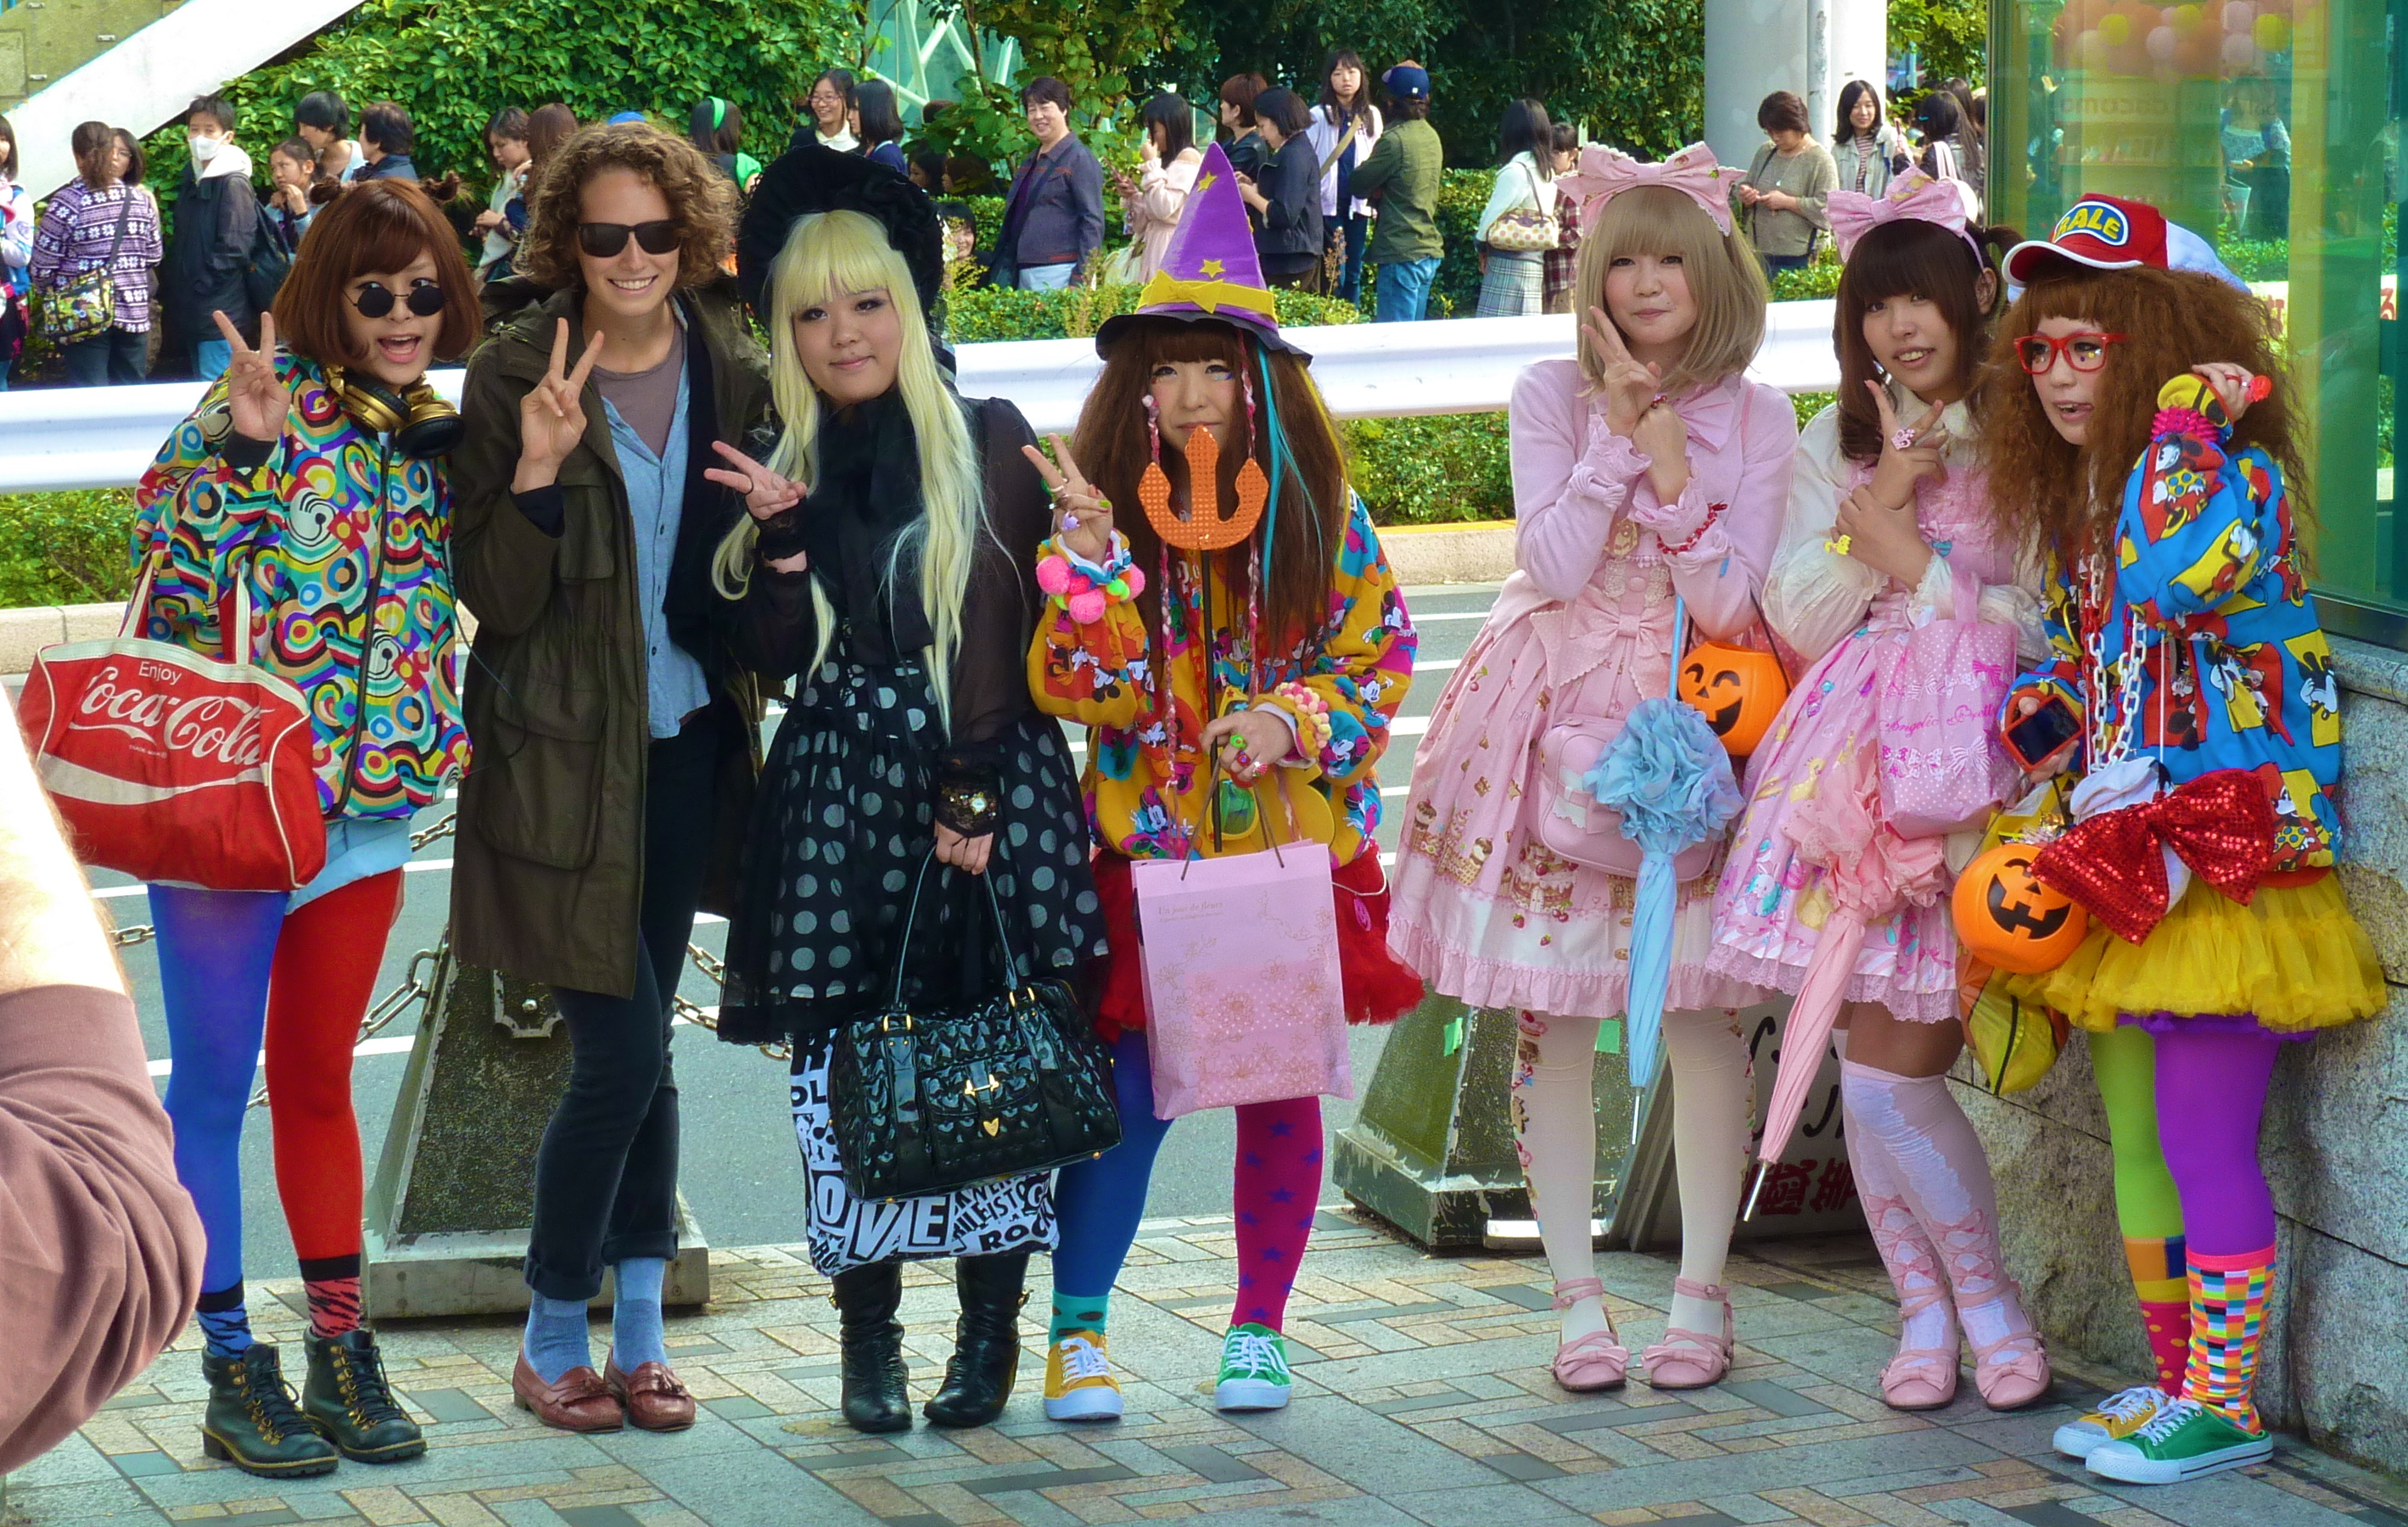
\includegraphics[height=0.25\textwidth]{photos/11/01/p10101771.jpg}}}
\end{figure}

\end{content}
\end{post}
